\documentclass[11pt, a4paper]{article}

\usepackage{anyfontsize}
\usepackage{txfonts} 
\usepackage{booktabs}
\usepackage{array}
\usepackage{geometry}
\usepackage{graphicx}
\graphicspath{{img/}}
\geometry{left=3cm,right=2.5cm,top=3.5cm,bottom=4cm}

%Graphics preamble
\usepackage{graphicx} %Allow you to import images
\usepackage{float} %Allow for control of float position

%Header and Footer Stuff
\pagestyle{myheadings}\markboth{page \thepage}{\emph Software Design Document}

%Table
\setlength{\arrayrulewidth}{0.5mm}

\begin{document}

\begin{titlepage}

\begin{center}

	\vspace{0.5 cm}
	\fontsize{35}{35}\selectfont\bf {Software Design Document}\\
	\vspace{0.5 cm}
	\huge{\bfseries for}\\
	\vspace{0.5 cm}
	\fontsize{35}{40}\selectfont\bf {Mesa Mapping Robot}\\
	
	\vspace{2cm}
	\Large\textbf{ Version 2.0 approved}\\
	
	\vspace{1.5cm}
	\Large\textbf {Prepared by SEP Group 19 - Spark\\
								Luo Yawen a1657343 \\
								Wei Jingwen a1671836 \\
								Wang Yuzhu a1690773 \\
								Yang Jiajun a1662541\\
								Zhang Yun a1653772}\\
		
	\vspace{2cm}
	\Large\textbf{ School of Computer Science,\\
								The University of Adelaide}\\
	\vspace{2cm}
	
	\Large\textbf{ Nov 01, 2015}\\

\end{center}

\end{titlepage}

%This is table of contents stuff
\pagenumbering{roman}
\tableofcontents

%This is the version history stuff
\vspace{1cm}
\section*{Revision History}
\addcontentsline{toc}{section}{\numberline{}Revision History}
%\begin{table}
\small
\begin{tabular} 
	 {|m{3cm}|m{2cm}|m{8cm}|m{2cm}|}
	\hline
	\textbf{Name} &  \textbf{Date} & \textbf{Reason For Changes} & \textbf{Version} \\ [0.5ex]
	\hline
	Wang Yuzhu & 21/Sep/15 & Add section 4 & 0.1\\ [0.5ex]
	\hline
	Wang Yuzhu & 24/Sep/15 & Add section 5 & 0.2 \\ [0.5ex]
	\hline
	Yang Jiajun & 29/Sep/15 & Add section 3 & 0.3 \\ [0.5ex]
	\hline
	Luo Yawen & 4/Oct/15 & Add section 6 & 0.4 \\ [0.5ex]
	\hline
	Luo Yawen & 6/Oct/15 & Add section 2 \& 7 \& 8 & 0.7 \\ [0.5ex]
	\hline
	Wang Yuzhu & 7/Oct/15 & Add section 1.1 \& 1.2 \& 1.3 & 0.8 \\ [0.5ex]
	\hline
	Yang Jiajun & 7/Oct/15 & Add section 1.4 \& 1.5 & 0.9\\ [0.5ex]
	\hline
	Luo Yawen & 7/Oct/15 & Release & 1.0 \\ [0.5ex]
	\hline
	Wang Yuzhu & 27/Oct/15 & Update 4 \& 5 & 1.4 \\ [0.5ex]
	\hline
	Yang Jiajun & 28/Oct/15 & Update 3  & 1.6 \\ [0.5ex]
	\hline
	Luo Yawen & 29/Oct/15 & Update 6 & 1.8 \\ [0.5ex]
	\hline
	Luo Yawen \newline Wang Yuzhu \newline Yang Jiajun & 30/Oct/15 & Review & 1.9 \\ [0.5ex]
	\hline
	Luo Yawen & 01/Nov/15 & Final release & 2.0 \\ [0.5ex]
	\hline
	
\end{tabular}
%\end{table}
\cleardoublepage

\newpage


%This is main body stuff
\pagenumbering{arabic}
\setcounter{page}{1}

%Section 1
\section{Introduction}

\subsection{Purpose}
This document sets out the software design base on the Software Requirements Specification document for the Mesa Mapping robot to be used for the Software Engineering and Project assignment for the University of Adelaide. Within this document, the System Architecture Design, Components Design, Data Design and Human Interface Design are set out for the Robot System, which will be implemented, in the second semester of 2015. Within this Software Design Document (SDD) will be the description for the detailed design of this system.

\subsection{Scope}
The system is for the surveying of a map, which will be done by a Lego Mindstorms EV3 robot. Two main purposes of the system are described in this document. The first purpose is to find the markings through the navigation of the robot on the survey map. The second purpose is to map an accurate map of the survey area by the robot. \\
\\
This document is a description of the design of the Mesa Mapping robot system, providing definitive guidance on the design of the Mesa Mapping robot system. Within this document the requirements documented in the Software Requirements Specification (SRS) will be reflected. 

\subsection{References}
Software Requirements Specification\\
SVN: \\
https://version-control.adelaide.edu.au/svn/SEPADL15S2PG19/\\
\\
Software Design Document (template): \\
https://forums.cs.adelaide.edu.au/mod/folder/view.php?id=22207\\
\\
Software Engineering and Project (2015):\\
https://forums.cs.adelaide.edu.au/pluginfile.php/46004/block\_html/content/ProjectDescription\_2015sem2.pdf

\subsection{Overview}
For this SDD document, firstly, we have a brief introduction of the content and design of the mapping robot system. After that, in section three, it contains a detailed description of the system architecture and components design. As for the section four, we utilise the UML (Unified Modelling Language) to identify the data design of the mapping robot system. Finally, some design details are referred in section five and six, among them, the human interface design is focused because the robot needs to be controlled through the GUI.

\subsection{Constraints}
If the distance between colour sensor and the object is too far, the detecting result would be unreliable. For this reason, it will affect the system to determine what next process the robot should take when detecting colours.\\
\\
The robot move through the track, so it would slip when it move on a slippy floor. It may influence the speed controlling.\\
\\
The code language is required to use Java by the client. Therefore, the appearance of the GUI may be a little different from the design version because Java is not so good for GUI development.

%Section 2
\section{System Overview}
Our system is designed for Lego Mindstorms EV3 robot project, which includes power, communication, mapping and movement four main subsystems. Each subsystem will satisfy on or more requirements according to the Software Requirements Specification (SRS). In this section, we will briefly introduce our system context and design. Besides, further details of our system will be mentioned in the next sections.\\
\\
For power system, it is used to work for the robot that make sure it can work when the user needs. And for communication system, which because the data in this system should be synchronous shared with all processes in this project. Then, for mapping system, it is used to work for map the survey area terrain. Last one is movement system, it is used to work for the react of robot.

%Section 3
\section{System Architecture and Components Design}
For this section, it mainly focuses on the system architecture and components design. Firstly, the system architecture will be shown through a figure. Then, the content is about component decomposition description. After that is detailed introduction of the components design. Finally, the content is the design rationale and an alternative system architecture.

\subsection{Architectural Description}
%Here we insert our figure
\begin{figure}[H]
\centering
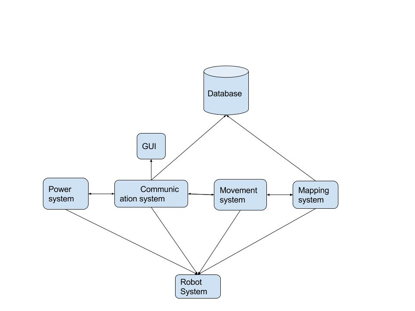
\includegraphics[height=4in]{SS}
\caption[Software system]{Software system}
\end{figure}

In this project, our software system mainly contains four subsystems, namely power system, communication system, mapping system and movement system. The system architecture diagram is shown above.

\subsection{Component Decomposition Description}
Power system: The power system is designed to control the power system of the mapping robot. In addition, it will show the dump energy to the user through GUI.\\
\\
Communication system: The communication system is responsible for bridging the user and the mapping robot. It will help the robot to receive orders from the user through Bluetooth. After receiving the order, the robot will call the corresponding reaction through movement system. \\
\\
Movement system: The movement system has the ability to receive orders from the communication system and control the robot to react accordingly. In addition, the movement of the robot is realised by two hardware subsystems including sensor system and engine system. The engine system contains one medium and two large motors, which are utilised to offer driving force to the robot. The sensor system contains four sensor that can help the robot react as expected (Such as move straightly, rotate 90 degrees and avoid the NGZ etc.).  \\
\\
Mapping system: The mapping system is designed for mapping. It can receive data from the movement system and control the sensor system to collect data. After that, the mapping system can record those data and map accordingly. Finally, the mapping information will store in database.\\
\\
Furthermore, the mapping system is eligible with the ability to load related map information data from the database.\\

\subsection{Detailed Components Design Description}
\textbf{Movement Component:}
\begin{itemize}
\item {\bfseries Purpose: }The movement component is designed to meet the operation requirement of the SRS (From R001 to R006).
\item {\bfseries Function: }The movement component can start and stop the robot, offer manual and automatic operation ways for the user to control the robot.
\item {\bfseries Subordinates: }Engine component and sensor component.
\item {\bfseries Dependencies: }This component will need order information from communication component while the robot is in manual model. When the robot is in the manual model, it will have no action unless receiving order from users. As required, the orders will only send through GUI by users.\item {\bfseries Interfaces: }The movement component needs orders from communication component while the robot is in manual model. Thus, an interface exists for receiving order data.
\item {\bfseries Data: }The speed data of the robot. Besides, the real-time position data will be recorded by this component. In the meantime, the real-time position data will send to mapping subsystem as soon as recording.
\end{itemize}
\\
\textbf{Communication Component:}
\begin{itemize}
\item {\bfseries Purpose: }The movement component is designed to meet the requirement of the SRS from R007 to R009, as well as R0017.
\item {\bfseries Function: }The communication component will mainly be responsible for human-computer interaction. It can show the real-time status of the robot to the user through GUI. In addition, orders can be collected through this component and then, sent to the movement component and power system. For example, a user chooses the automatic mapping function and after completing, turns off the power button on the GUI. The communication component will collect the orders sent by the user, and then sent the automatic mapping order to the movement component and after completing, sent power off order to the power system to turn off the robot.
\item {\bfseries Subordinates: }Login-out component, which will verify the authority of the user.
\item {\bfseries Dependencies: } This component is linked to the GUI, and it will receive orders from users through GUI and sent the orders to the movement component and the power system.
\item {\bfseries Interfaces: }This component will offer the order data to the movement component and power system. In addition, it will receive order information which given by users through GUI. So it has three interfaces, one is used to collect order information from GUI. Another two are utilized to send the orders to the movement system and power system.
\item {\bfseries Data: }Order data given by users through GUI.
\end{itemize}
\\
\textbf{Mapping Component:}
\begin{itemize}
\item {\bfseries Purpose: }The movement component is designed to meet the requirement of the SRS from R0010 to R0013. 
\item {\bfseries Function: }This component has the ability to load and save the survey map. In addition, it can set or cancel the NGZ.
\item {\bfseries Subordinates: }Sensor component.
\item {\bfseries Dependencies: }This component is linked to the movement component. It will receive the real-time position data from the movement component and map accordingly.
\item {\bfseries Interfaces: }This component has an interface with the movement component for receiving real-time position data, barrier data etc.
\item {\bfseries Data: }Map data (Such as the position data, the NGZ data etc.). The related data is recorded by movement component. 
\end{itemize}
\\
\textbf{Login-out Component:}
\begin{itemize}
\item {\bfseries Purpose: }The login-out component is designed to meet the requirement of the SRS from R0014 to R0016. 
\item {\bfseries Function: }This component is designed for checking the authority of the user.
\item {\bfseries Subordinates: }No.
\item {\bfseries Dependencies: }This component is designed for checking the authority of the user.
\item {\bfseries Interfaces: } This component will verify the user's authority and send it to the communication component to determine the permit operation.
\item {\bfseries Data: }User's information data.
\end{itemize}
\\
\textbf{Sensor Component:}
\begin{itemize}
\item {\bfseries Purpose: }The sensor component is designed control the sensors and collect data when mapping. It links to the requirement of the SRS from R0010 to R0013. 
\item {\bfseries Function: }This component is designed for controlling the sensors and collecting data.
\item {\bfseries Subordinates: }No.
\item {\bfseries Dependencies: }This component is the subordinate of the mapping and movement components. It will offer data to these two components and receive orders back.
\item {\bfseries Interfaces: }This component has interfaces with mapping and movement components for exchanging data and order.
\item {\bfseries Data: }Colour data, direction data and distance data.
\end{itemize}
\\
\textbf{Engine Component:}
\begin{itemize}
\item {\bfseries Purpose: }The engine component is designed to offer drive force of the robot. It links to the requirement of the SRS R006.
\item {\bfseries Function: }This component is designed help the robot to move.
\item {\bfseries Subordinates: }No.
\item {\bfseries Dependencies: }This component is the subordinate of the movement components which will deliver orders to it.
\item {\bfseries Interfaces: }This component has interfaces with the movement component for receiving orders.
\item {\bfseries Data: }Speed data from the movement component.
\end{itemize}
\\
\textbf{Power Component:}
\begin{itemize}
\item {\bfseries Purpose: }To control the power of the robot. Thus realise the function that the user can turn on/off the robot through GUI.
\item {\bfseries Function: }This component is designed to control the power of the robot. In addition, it can display the dump energy on GUI.
\item {\bfseries Subordinates: }No.
\item {\bfseries Dependencies: }This component will receive energy related order through the communication component. 
\item {\bfseries Interfaces: }This component will sent the real-time dump energy information to the communication component and also receive energy related order from it. Thus, it has an interface to link with the communication component.
\item {\bfseries Data: }Energy related orders (such as turn on/off the robot) and real-time dump energy.\end{itemize}

\subsection{Architectural Alternatives}
If the existing software architecture design is too trivial, we will merge some subsystem. For example, we would merge the power system to the communication system. If possible, communication system and movement system would be merged to one system because these two systems are tightly connected. 

\subsection{Design Rationale}
First, we take the requirement of the RSR into consideration. Then we design the mapping system, movement system and communication system because these three system can perfectly cover all main requirements. Furthermore, another reason is that the interaction of them is clear. \\ 
\\
In addition, because the rest time is limited and only three members of us are mainly responsible for code, we designed this kind of architecture with four main subsystems. Among these four subsystems, one person will responsible for the power system and communication system because these two systems are relatively simple. As for the movement and mapping systems, they will be controlled by the rest two people separately. 
\newpage

%Section 4
\section{Data Design}
In this section, the data description and data structures, which implemented in the Robot Mapping System will be described. Data description describes briefly about the database. The detailed database design, including entities and their relationships will be given in the data structures part.

\subsection{Database Description}
The Database Management System (DBMS) Access will be used in the Robot Mapping System. The database will support the Robot Mapping System to store and organise the information about the user, map, message and help. \\
\\
The Data Structures part descripts the relationship among the tables. There are 7 tables used in this project, they are descripted in User Information part, Map Information part, Message Information part and Help Information part separately. Each part will provide the table design and explain what are the tables for and what are the item for in each table. By reading this part, software developers could implement the database of the system. \\

%Here we insert our figure
\begin{figure}[H]
\centering
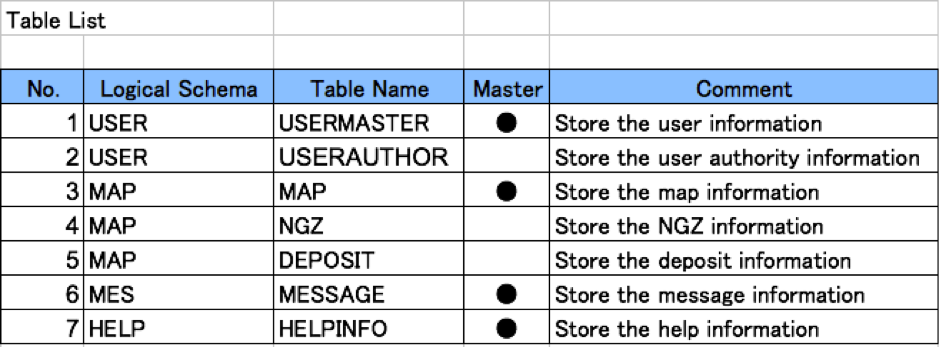
\includegraphics[height=2.3in]{TL}
\caption[Table List]{Table List}
\end{figure}
\newpage

\subsection{Data Structures}
The data structures organise the items stored and the relationship with each other in the Robot Mapping system. This data structure includes User Info data structure, Map Info data structure, Message Info data structure and Help Info data structure. Each entity will include the enter time, enter user, update time and update user.

%Here we insert our figure
\begin{figure}[H]
\centering
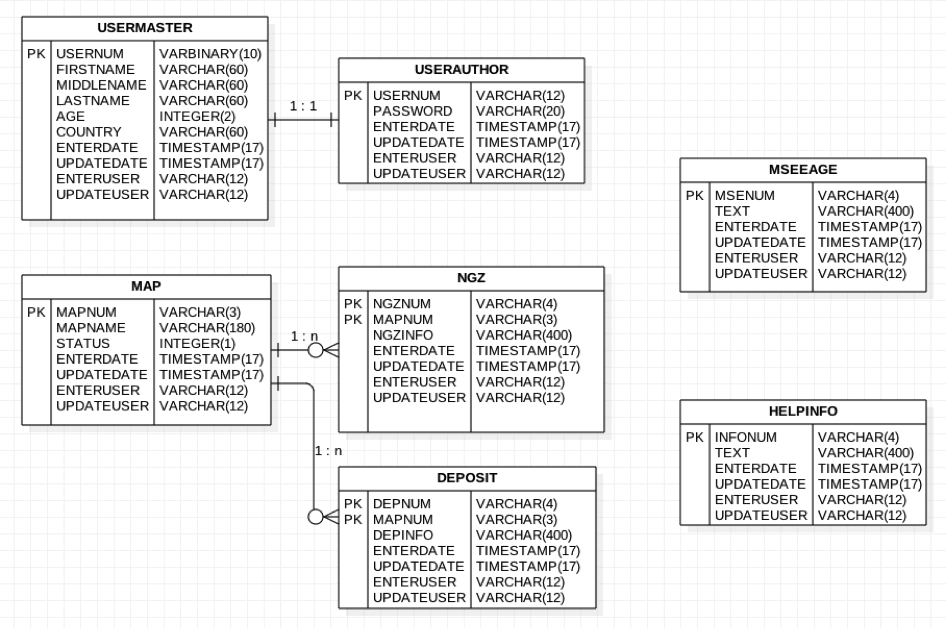
\includegraphics[height=3.6in]{DS}
\caption[Data Structures]{Data Structures}
\end{figure}

\subsubsection{User Information}
There are two entities in User Info data structure to store the operator's information and check the authority of each operator. User master will store the basic information of the user, including name, age and country. Each user will have his own user number and password, the password will be stored in user author entity, the relationship between user master and user author is 1 to 1 connected by the primary key user number. These entities will be used in user login author check function.

%Here we insert our figure
\begin{figure}[H]
\centering
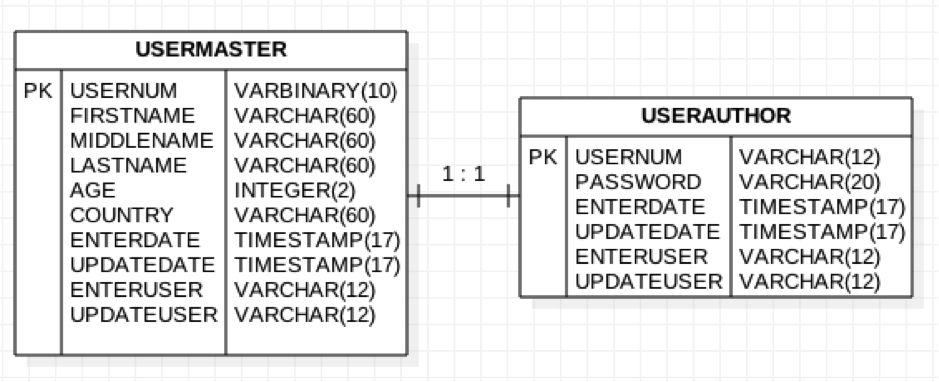
\includegraphics[height=2in]{UI}
\caption[User Info Tables]{User Info Tables}
\end{figure}

%Here we insert our figure
\begin{figure}[H]
\centering
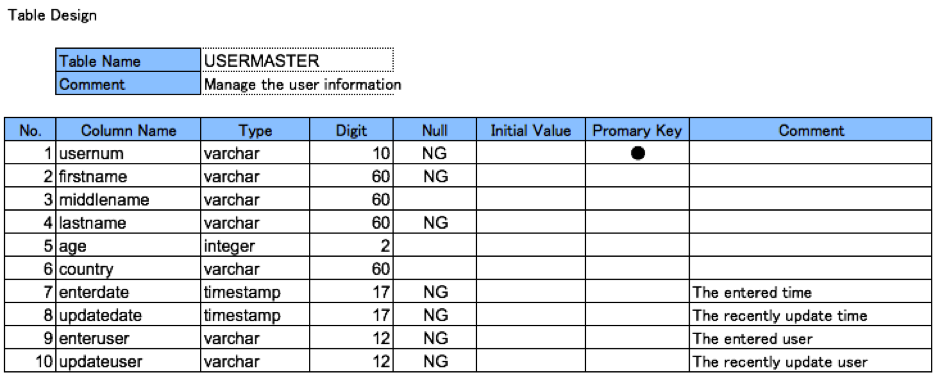
\includegraphics[height=2.5in]{USM}
\caption[Table design USERMASTER]{Table design USERMASTER}
\end{figure}

%Here we insert our figure
\begin{figure}[H]
\centering
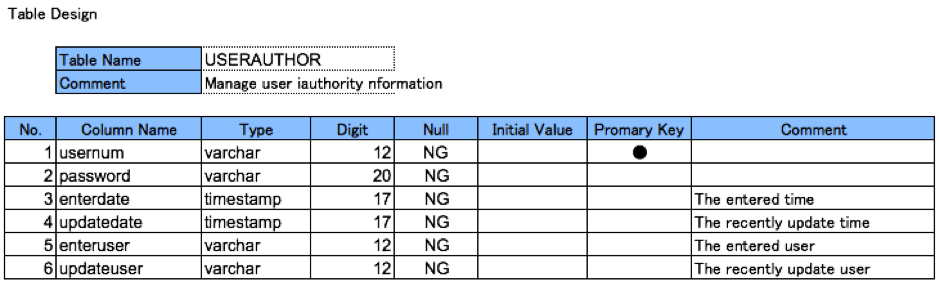
\includegraphics[height=2in]{USA}
\caption[Table design USERAUTHOR]{Table design USERAUTHOR}
\end{figure}

\subsubsection{Map Information}
There are three entities in Map Info data structure to store the Map Info. Each map will have three kinds of status, 1 (completed), 2 (in process) and 3 (unsurvey). There will be the NGZ Info and Deposit Info for the map which status is 1 or 2.\\
\\
Each map may have more than one NGZ and deposits, the information will be stored in the NGZ entity and the deposit entity. The relationship between the map entity and the NGZ entity will be 1 to n, connected by the primary key map number. The relationship between the map entity and the deposit entity will be 1 to n, connected by the primary key map number. 

%Here we insert our figure
\begin{figure}[H]
\centering
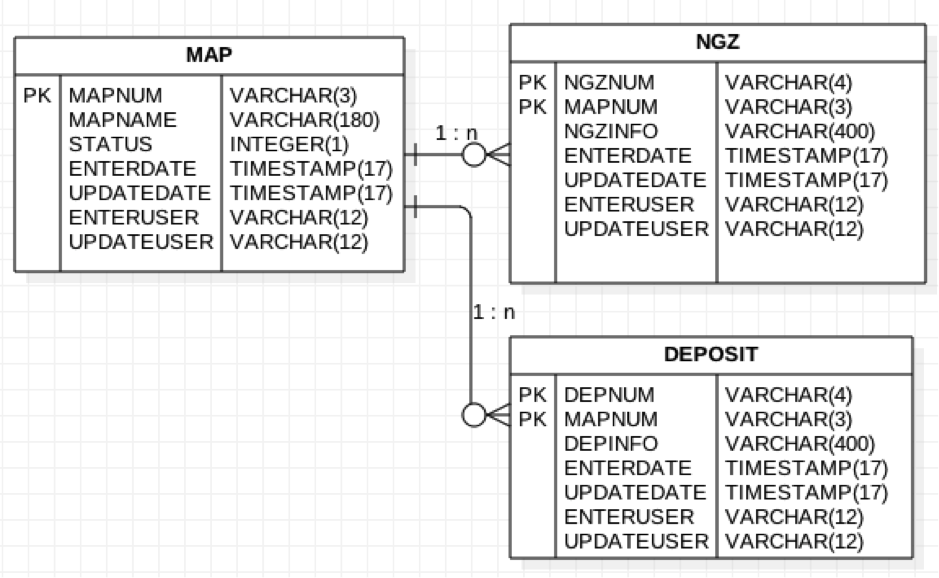
\includegraphics[height=3in]{MI}
\caption[Map Info]{Map Info}
\end{figure}

%Here we insert our figure
\begin{figure}[H]
\centering
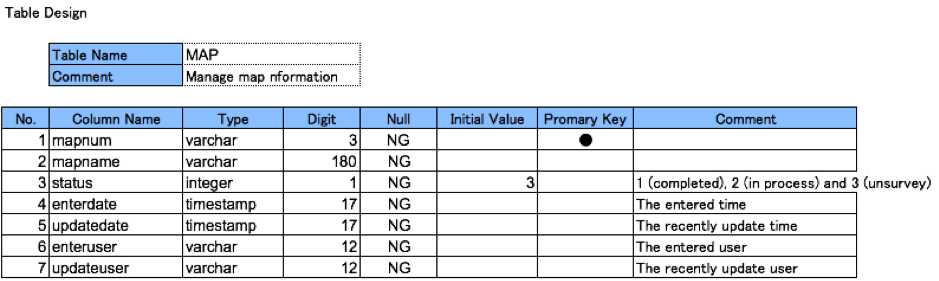
\includegraphics[height=2in]{DM}
\caption[Table design Map]{Table design Map}
\end{figure}

%Here we insert our figure
\begin{figure}[H]
\centering
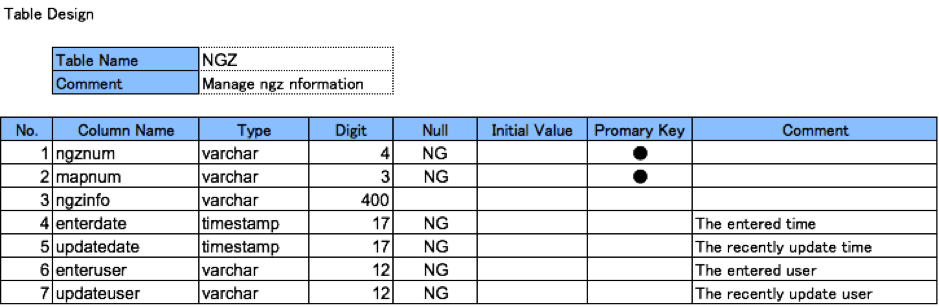
\includegraphics[height=2in]{NGZ}
\caption[Table design NGZ]{Table design NGZ}
\end{figure}

%Here we insert our figure
\begin{figure}[H]
\centering
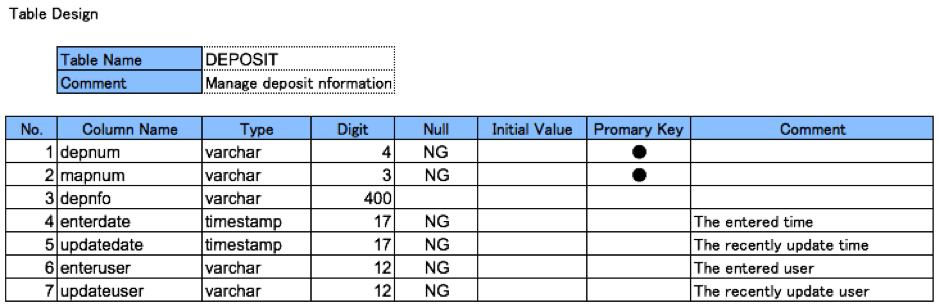
\includegraphics[height=2in]{DE}
\caption[TTable design DEPOSIT]{Table design DEPOSIT}
\end{figure}

\subsubsection{Message Information}
Message entity stores the detail about each message that the robot sends to the operator. The robot will send message number to the operation system, then the system will search the content of the message from this entity. The primary key of this entity is message number.

%Here we insert our figure
\begin{figure}[H]
\centering
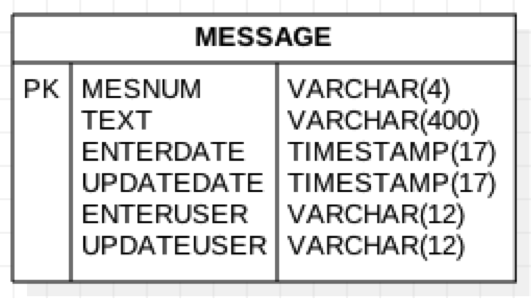
\includegraphics[height=2in]{MIN}
\caption[Message Info]{Message Info}
\end{figure}

%Here we insert our figure
\begin{figure}[H]
\centering
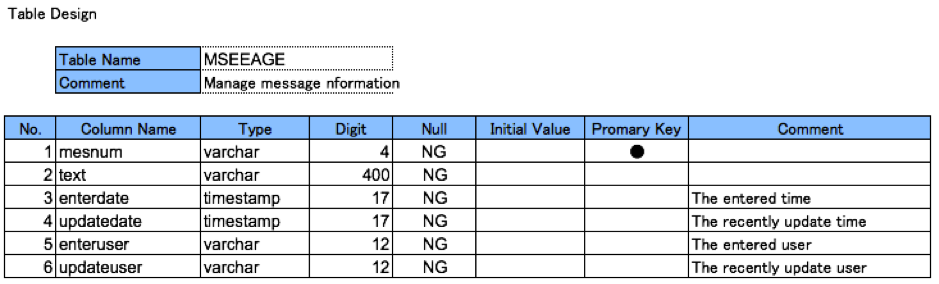
\includegraphics[height=2in]{ME}
\caption[Table design Message]{Table design Message}
\end{figure}

\subsubsection{Help Information}
Help Info entity stores the detail about help information. Each help information will be numbered by the primary key info number and the content of the message will be stored in the text attribute. The primary key of this entity is info number. This entity will be used in the user help function.

%Here we insert our figure
\begin{figure}[H]
\centering
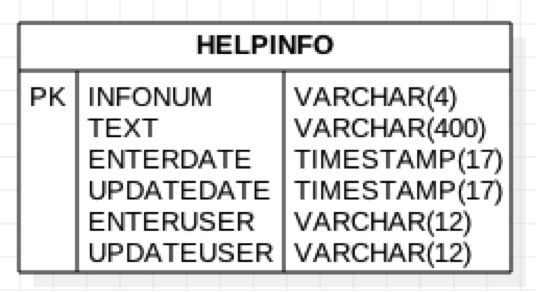
\includegraphics[height=2in]{HI}
\caption[Help Info]{Help Info}
\end{figure}

%Here we insert our figure
\begin{figure}[H]
\centering
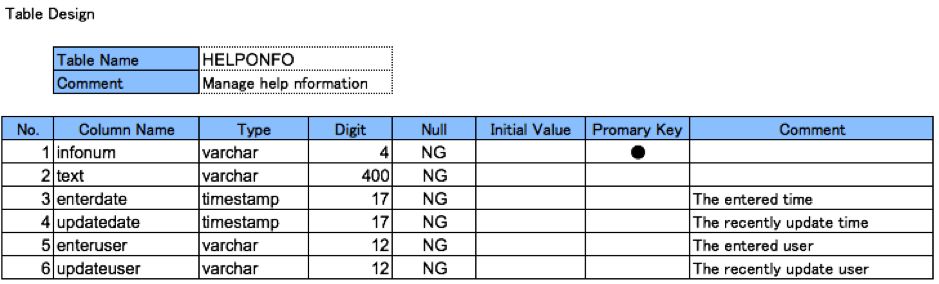
\includegraphics[height=2in]{HE}
\caption[Table design HELPINFO ]{Table design HELPINFO }
\end{figure}
\newpage

%Section 5
\section{Design Detail}
This section describes the design details, including classes considered in the system, all the states of the robot and the interactions between each function. The design will be described by class diagram, state diagram and interaction diagram.

\subsection{Class Diagrams}
This diagram describes all the class diagrams considered in the Robot Mapping system. This diagram reflects the requirements documented in the SRS. Associated details in these diagrams are including class name, attributes and methods.\\

%Here we insert our figure
\begin{figure}[H]
\centering
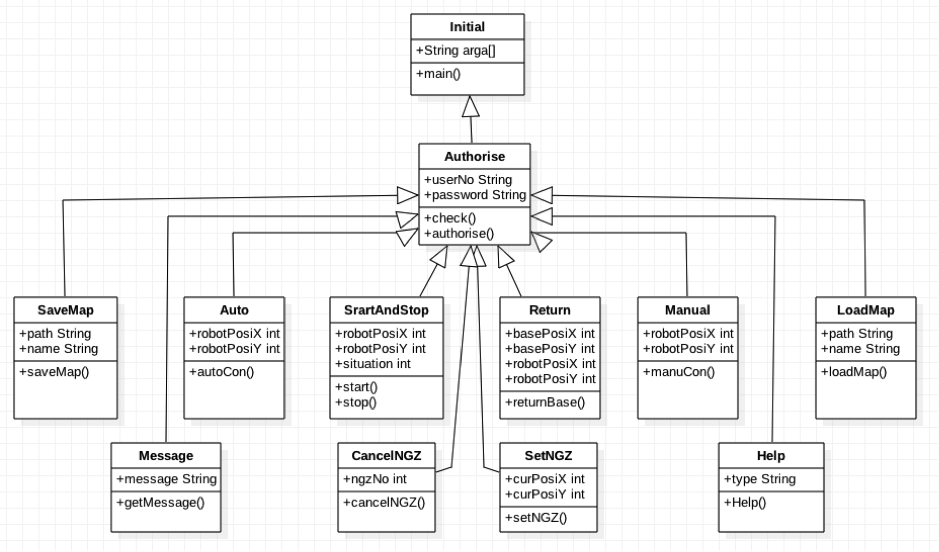
\includegraphics[height=4in]{CD}
\caption[Class Diagram]{Class Diagram}
\end{figure}
\newpage

%5.1.1
\subsubsection{Authorise}
\begin{itemize}
\item {\bfseries Responsibilities }\\
This method will check the authority of the login user. If the check is successful the user can operate the robot, otherwise there will be an error message (MSEID:001) showed in the login screen.\\

\item {\bfseries Interface }\\
1. Input: UserNum (varchar 10), Password (varchar 20)\\
2. Output: 0 (Authorise Check OK), 1 (Authorise Check NG)\\


\item {\bfseries Database }\\
1. USERMASTER (Figure 4-4)}\\
2. USERAUTHOR (Figure 4-5)}\\
3. MESSAGE (Figure 4-11)}\\

\item {\bfseries Interaction }\\
Input the UserNum and Password, then put the login button on the login screen.\\

\item {\bfseries Processing }\\
1. Check the type of the UserNum and Password\\
1.1 If the input UserNum is null, then return an error message (MESID:002) to the login screen. If or Password is null, then return an error message (MESID:003) to the login screen.\\
1.2 If the input UserNum is not varchar type or the digit is longer than 10, then return an error message (MESID:004) to the login screen.\\
1.3 If the input Password is not varchar type or the digit is longer than 20, then return an error message (MESID:004) to the login screen.\\
\\
2. Check the authority of the login user\\
Select the password by using the input parameter usernum from USERMASTER table and USERAUTHOR, if the password get from DB equals the input parameter password, then check OK (return 0). Otherwise NG (return 1).\\

\item {\bfseries Message }\\
All the messages are stored in the MESSAGE entity.\\
\\
MSE 001: Incorrect Username or Password\\
MSE 002: Please input the UserName\\
MSE 003: Please input the Password\\
MES 004: Forbidden character\\
\end{itemize}

%5.1.2
\subsubsection{Start and Stop}
\begin{itemize}
\item {\bfseries Responsibilities }\\
This method will implement the start function and stop function of the robot. There will be a button on the screen, when it presents as start the user can push the button to start the robot, then the button will change to present as stop, then the user can stop the robot by pushing this button again.

\item {\bfseries Interface }\\
1. Input: coordinate X, coordinate Y\\
2. Output: 0 (start), 1 (stop), 2 (error)\\

\item {\bfseries Database }\\
None

\item {\bfseries Interaction }\\
1. User put the start button on the main screen will start the robot.\\
\\
2. User put the stop button on the main screen will stop the robot.\\

\item {\bfseries Processing }\\
1. Start\\
Check the situation of the robot, including energy, the security and the position.
If check is ok, then start the robot and return 0, else send an error message (005) to the screen and return 2.\\
\\
2. Stop\\
Check the situation of the robot, including the security and the position.
If check is ok, then stop the robot and return 1, else send an error message (006) to the screen and return 2.\\

\item {\bfseries Message }\\
All the messages are stored in the MESSAGE entity.\\
\\
MSE 005: The robot cannot be started\\
MSE 006: The robot cannot be stopped\\
\end{itemize}

%5.1.3
\subsubsection{Save Map }
\begin{itemize}
\item {\bfseries Responsibilities }\\
This method will implement the save map function of the robot. The user can save the map any time when the robot is stopped. However, the map cannot be save when the robot is working.

\item {\bfseries Interface }\\
1. Input: MapNum\\
2. Output: Message\\

\item {\bfseries Database }\\
1. MAP (Figure 4-7)\\
2. NGZ (Figure 4-8)\\
3. DEPOSIT (Figure 4-9)\\
4. MESSAGE (Figure 4-11)\\

\item {\bfseries Interaction }\\
When the user puts the save map button on the main screen, the surveying map will be saved.\\

\item {\bfseries Processing }\\
1. Check the robot, if the robot is working, then send an error message (007).\\
\\
2. Update database\\
2.1 Update the status in MAP entity\\
2.2 Insert NGZ entity if there is NGZ on the map\\
2.3 Insert DEPOSIT entity if there is deposit on the map\\
\\
3. Save the map to the location which the user chooses. If the operation is successful return message (008) else return message (009).\\

\item {\bfseries Message }\\
All the messages are stored in the MESSAGE entity.\\
\\
MSE 007: Please stop the robot before saving the map\\
MSE 008: The map has been saved\\
MSE 009: The map cannot be saved\\
\end{itemize}

%5.1.4
\subsubsection{Load  Map }
\begin{itemize}
\item {\bfseries Responsibilities }\\
This method will implement the load map function of the robot. The user can load the map any time when the robot is stopped. However, the map cannot be load when the robot is working.

\item {\bfseries Interface }\\
1. Input: None\\
2. Output: The loaded map\\

\item {\bfseries Database }\\
1. MAP (Figure 4-7)\\
2. MESSAGE (Figure 4-11)\\

\item {\bfseries Interaction }\\
When the user pushes the load map button on the main screen, the new map will be loaded.\\

\item {\bfseries Processing }\\
1. Check the robot, if the robot is working, then send an error message (007).\\
\\
2. Check whether there is a current map on the screen. If there is a map on the screen, then send a message (010).\\
\\
3. Load the map which the user chooses. If the operation is successful return message (011) else return message (012).\\
\\
4. If the operation is successful, insert MAP entity, set the status = 3.\\

\item {\bfseries Message }\\
All the messages are stored in the MESSAGE entity.\\
\\
MES 010: Do you want to delete the current map? \\
MES 011: The map has been uploaded.\\
MES 012: The map has not been uploaded.\\
\end{itemize}

%5.1.5
\subsubsection{Auto}
\begin{itemize}
\item {\bfseries Responsibilities }\\
This method will implement the auto survey function of the robot. The robot can survey the map automatically when the user switch survey mode to auto.\\

\item {\bfseries Interface }\\
1. Input: Mode (auto 1), coordinate X, coordinate Y\\
2. Output: None\\

\item {\bfseries Database }\\
None

\item {\bfseries Interaction }\\
By switching the survey mode to auto.\\

\item {\bfseries Processing }\\
When the robot is in the auto mode, the robot will survey the map according the exist survey method automatically, including not cross the boundary, not go to the NGZ, record the colour markings and survey the map line by line.\\

\item {\bfseries Message }\\
None
\end{itemize}

%5.1.6
\subsubsection{Manual}
\begin{itemize}
\item {\bfseries Responsibilities }\\
This method will implement the manual survey function of the robot. The robot can survey the map manually when the user switches survey mode to manual.\\

\item {\bfseries Interface }\\
1. Input: Mode (manual 2), coordinate X, coordinate Y\\
2. Output: None\\

\item {\bfseries Database }\\
None

\item {\bfseries Interaction }\\
The user can operation the robot by pushing the four operation buttons on the main screen to survey the area.\\

\item {\bfseries Processing }\\
When the robot is in auto mode, the robot will survey the user operation, including not cross the boundary, not go to the NGZ, record the colour markings.\\

\item {\bfseries Message }\\
None
\end{itemize}

%5.1.7
\subsubsection{Set NGZ }
\begin{itemize}
\item {\bfseries Responsibilities }\\
This method will implement the NGZ set function. The NGZ can be allocated during the survey dynamically. The robot must not enter the NGZ.\\

\item {\bfseries Interface }\\
1. Input: coordinate X, coordinate Y\\
2. Output: None\\

\item {\bfseries Database }\\
1. NGZ (Figure 4-8)\\

\item {\bfseries Interaction }\\
When the user pushes the NGZ set button on the main screen, the NGZ can be set on the map dynamically. The NGZ could be any colour and shape.\\

\item {\bfseries Processing }\\
1. NGZ set\\
1.1 Check the position of the robot, the NGZ cannot be set where the robot is.\\
1.2 Choose the NGZ colour.\\
1.3 Set the NGZ by setting the coordinate X and coordinate Y.\\
\\
2. Insert the NGZ information into NGZ entity.\\

\item {\bfseries Message }\\
None
\end{itemize}

%5.1.8
\subsubsection{Cancel NGZ }
\begin{itemize}
\item {\bfseries Responsibilities }\\
This method will implement the NGZ cancel function. The NGZ can be canceled during the survey.\\

\item {\bfseries Interface }\\
1. Input: NGZnum\\
2. Output: None\\

\item {\bfseries Database }\\
1. NGZ (Figure 4-8)\\

\item {\bfseries Interaction }\\
When the user pushes the NGZ cancel button on the main screen, the chosen NGZ can be canceled from the map.\\

\item {\bfseries Processing }\\
1. Cancel the NGZ from the map.\\
\\
2. Delete the NGZ information by the input from the NGZ entity.

\item {\bfseries Message }\\
None
\end{itemize}

%5.1.9
\subsubsection{Return to the base }
\begin{itemize}
\item {\bfseries Responsibilities }\\
This method will implement the return to the base station function. The robot will return to the base station automatically.\\

\item {\bfseries Interface }\\
1. Input: coordinate X, coordinate Y\\
2. Output: None\\

\item {\bfseries Database }\\
None

\item {\bfseries Interaction }\\
The user pushes the return button on the main screen.\\

\item {\bfseries Processing }\\
1. Use the position of the base station and the current position of the robot to calculate the path and the distance between the base station and the robot.\\
\\
2. Send an order to the robot, then the robot will return to the base station automatically.\\

\item {\bfseries Message }\\
None
\end{itemize}

%5.1.10
\subsubsection{Help}
\begin{itemize}
\item {\bfseries Responsibilities }\\
This method will implement the help function. This function is to help use to solve the problem when the user operates the robot and provide information to help user.\\

\item {\bfseries Interface }\\
None

\item {\bfseries Database }\\
1. NGZ (Figure 4-12)\\
2. MESSAGE (Figure 4-11)\\

\item {\bfseries Interaction }\\
By pushing the help button in main screen and NGZ set screen.\\

\item {\bfseries Processing }\\
Select the help information from the HELPINFO entity. 

\item {\bfseries Message }\\
None
\end{itemize}

\subsection{State Diagrams}
This diagram describes all the states of the robot considered in the Robot Mapping system. This diagram reflects the requirements documented in the SRS. \\
\\
The robot will have two states, starting and stopping. During the start state, the user can operate the robot to survey, when the robot returns to the base or the user presses the stop button, the robot will turn stop state.

%Here we insert our figure
\begin{figure}[H]
\centering
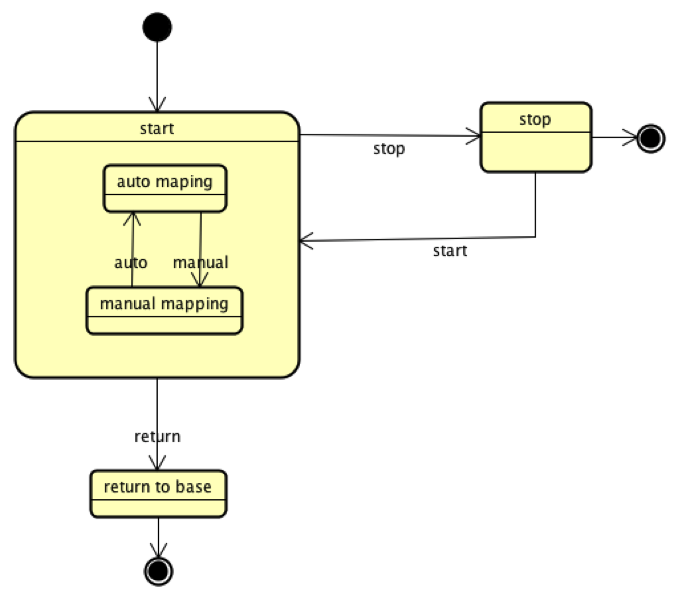
\includegraphics[height=3in]{SD}
\caption[State Diagram]{State Diagram}
\end{figure}

\begin{enumerate}
\item {The operations below can be implemented in start status.}\\
Survey the map, change the survey mode, set NGZ, cancel NGZ, return to the base.\\
\item {The operations below can be implemented in stop status.}\\
Change the survey mode, set NGZ, cancel NGZ, return to the base, save the map, load the map.\\
\end{enumerate}
\newpage

\subsection{Interaction Diagrams}
This diagram describes all the interactions considered in the Robot Mapping system. This diagram reflects the requirements documented in the SRS. This diagram also reflect the interaction mentioned in section 5.1.

%Here we insert our figure
\begin{figure}[H]
\centering
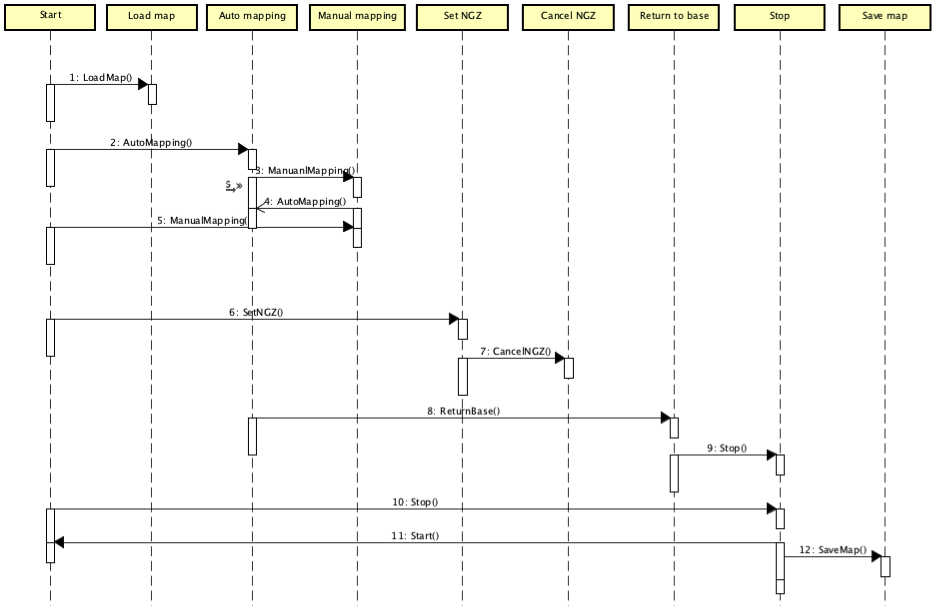
\includegraphics[height=4in]{ID}
\caption[Interaction Diagram]{Interaction Diagram}
\end{figure}
\newpage

%Section 6
\section{Human Interface Design}
In this section, we will describe our GUI of our system in detail. The GUI contains a single screen that used to display the map,and several buttons that used to execute corresponding functions.

\subsection{Overview of the User Interface}
The User will interface with the Robot through a GUI. The GUI shall use visible buttons to indicate available function that the robot able to execute. The quantitative action shall also have blanks for the user to fill in. \\
\\
The GUI of our program will include disconnect button, loading and saving map, returning to the base, the auto-manual switch and the status information of the robot. Loading and saving map will include the location, direction and track of the robot and the position of the deposit. The auto-manual switch shall also have distinct interface which will facilitate the user observe mode easily. Under the manual mode, the user can control the robot to do basic movement (forward/backward, turn left/right). In addition, the status of the robot will be display on the GUI which includes coordinates communicate messages and state of charge.

%Here we insert our figure
\begin{figure}[H]
\centering
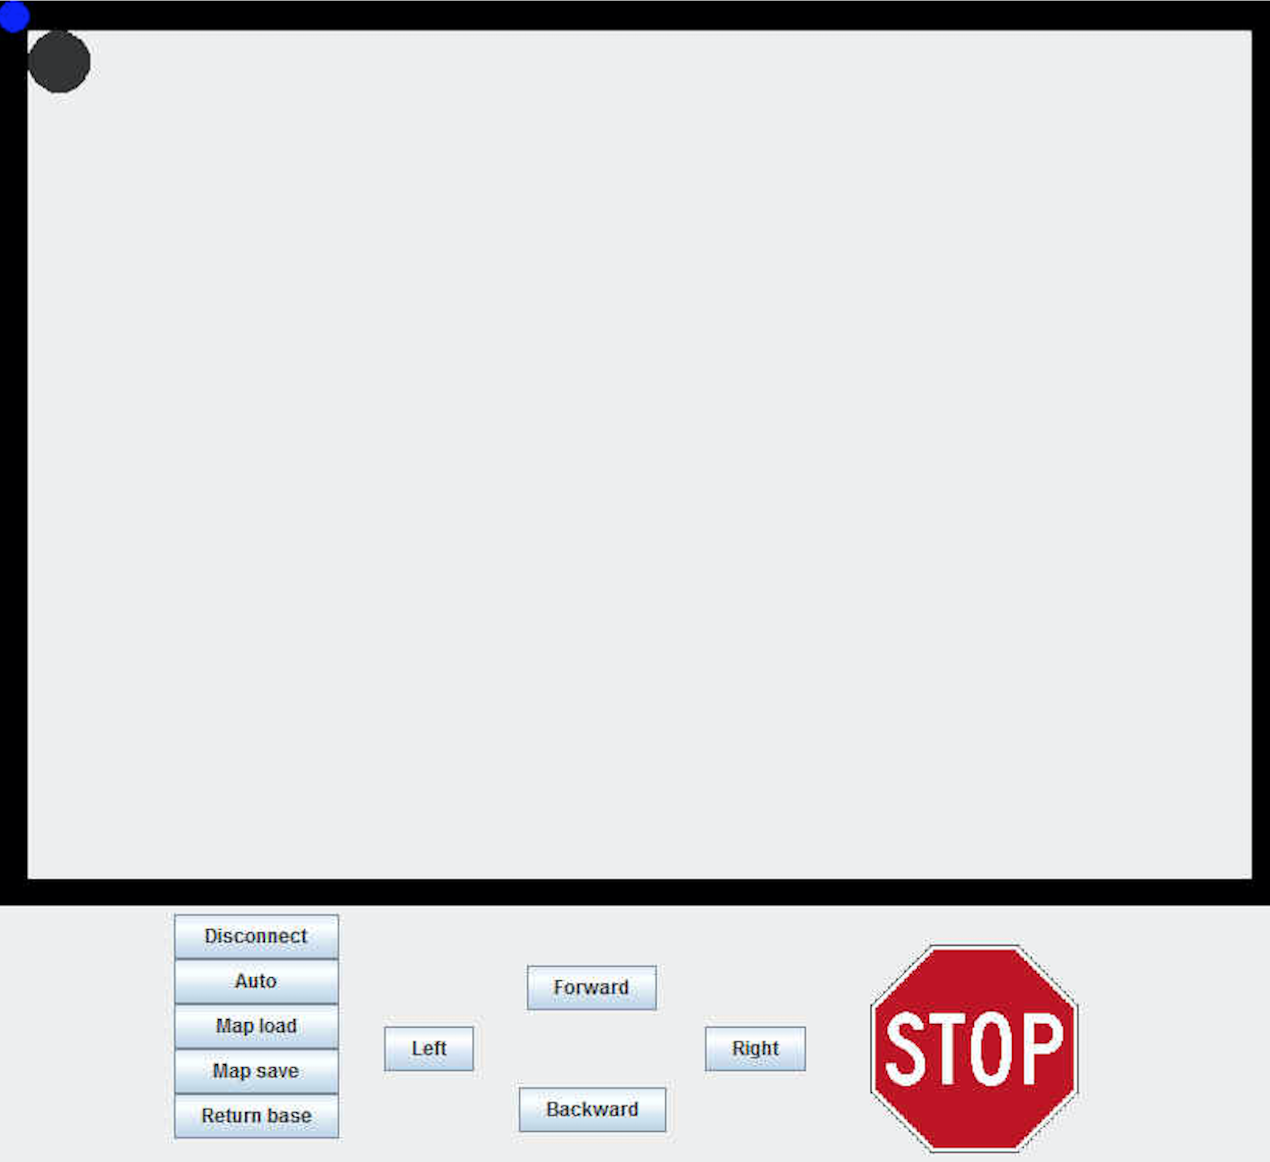
\includegraphics[height=5in]{main}
\caption[Main Interface]{Main Interface}
\end{figure}

\subsection{Detailed Design of the User Interface}
\subsubsection{Map}
This displays the map that is the place the robot works on, and the user can search the track of the robot, the current direction of robot, the location of each kind of deposit, communications tower and operations base, and the range of the NGZ based on the sensor detection.

%Here we insert our figure
\begin{figure}[H]
\centering
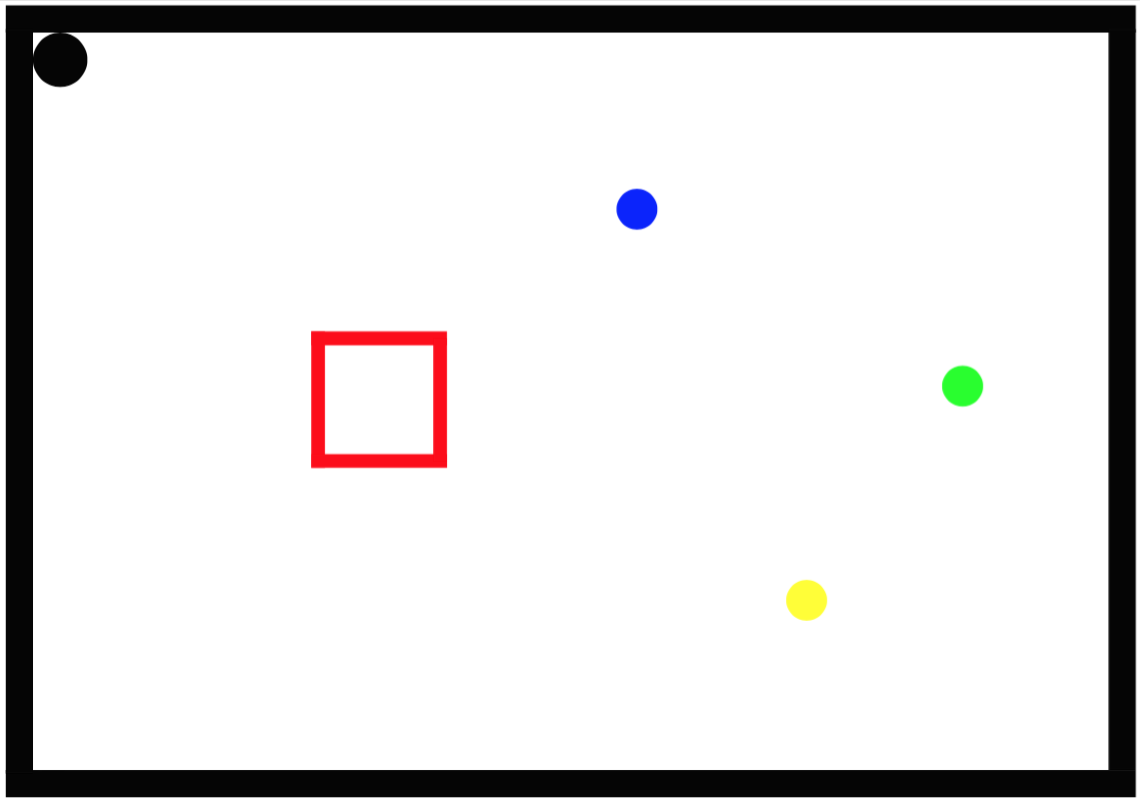
\includegraphics[height=3in]{map}
\caption[Map]{Map}
\end{figure}

\subsubsection{Status information}
This displays the position of robot in coordinates way during the robot working, communicate messages and state of charge, which to make sure the robot can work smoothly.

%Here we insert our figure
\begin{figure}[H]
\centering
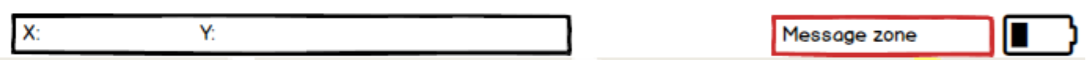
\includegraphics[height=0.3in]{SI}
\caption[Status information]{Status information}
\end{figure}
\newpage

\subsubsection{Buttons}
This includes the button of disconnect that can connect or disconnect between the robot and PC, the button of Loading and saving map that allow the user to load and save specific map, the button of retuning base that can allow robot to go back to the base, and the auto-manual switch is used to change the mode from automatic to manual.

%Here we insert our figure
\begin{figure}[H]
\centering
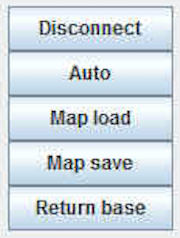
\includegraphics[height=3in]{buttons}
\caption[Buttons]{Buttons}
\end{figure}

\subsubsection{Direction function}
The four-arrow button is used to move the robot manually by the user (forward for moving forward, backward for moving backward, left for turning left, and right for turning right). And the stop button is used to stop the robot immediately.

%Here we insert our figure
\begin{figure}[H]
\centering
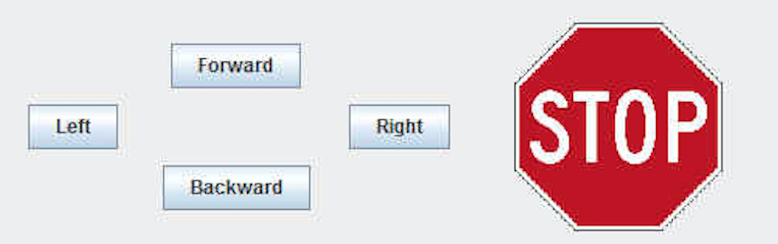
\includegraphics[height=2in]{auto}
\caption[Direction function]{Direction function}
\end{figure}
\newpage

\subsubsection{Map Load}
Users can use map load button to load the map, which is for the robot uses. The save map button will prompt the user with a save map dialog when the button is clicked.

%Here we insert our figure
\begin{figure}[H]
\centering
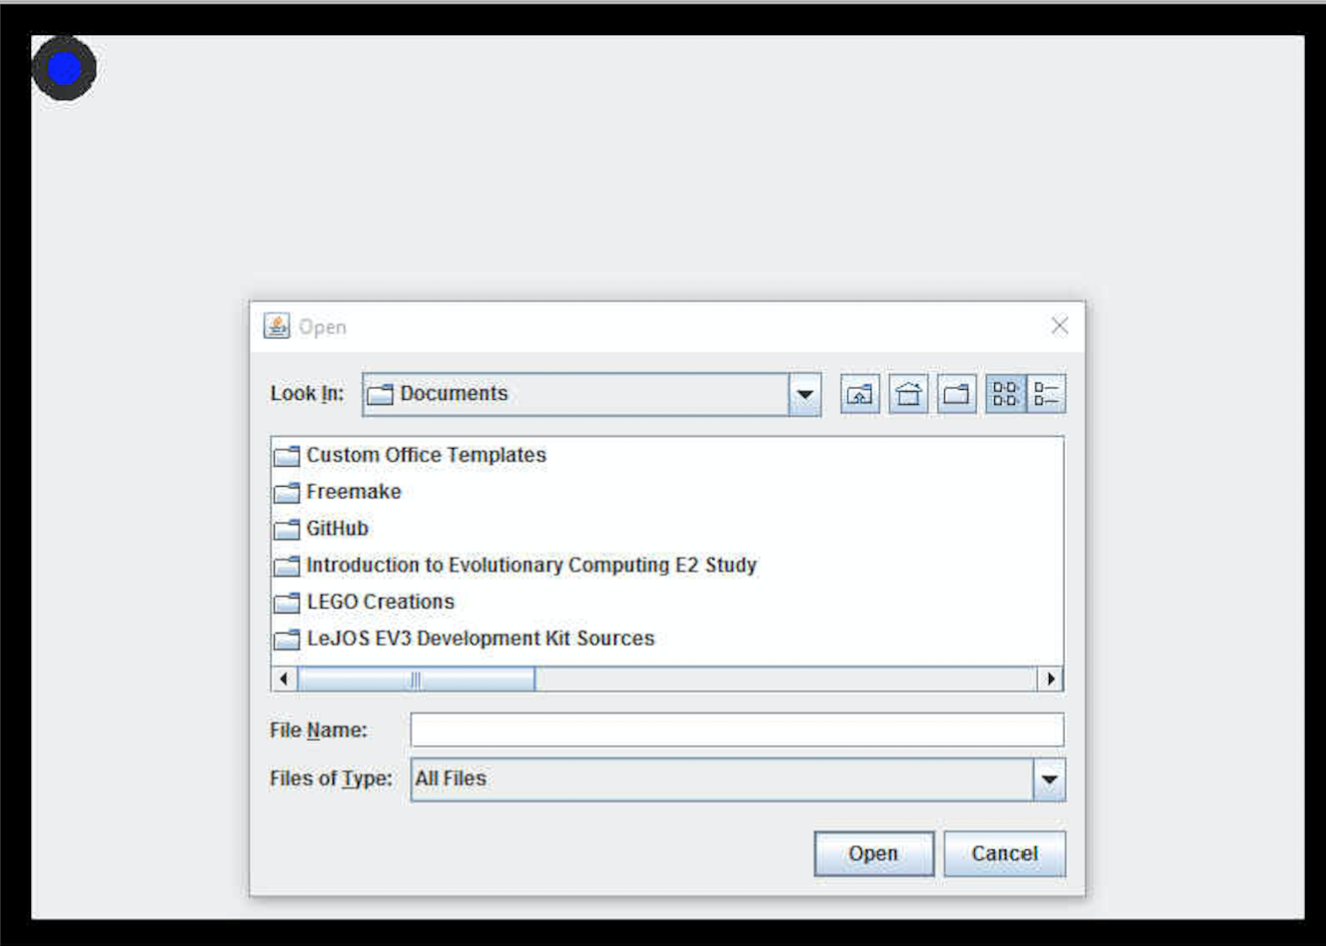
\includegraphics[height=3in]{load}
\caption[Map Load]{Map Load}
\end{figure}

\subsubsection{Map Save}
Users can use map save button to save current map, which is for the robot uses. The user will be able to save the current map file into a specific directory.

%Here we insert our figure
\begin{figure}[H]
\centering
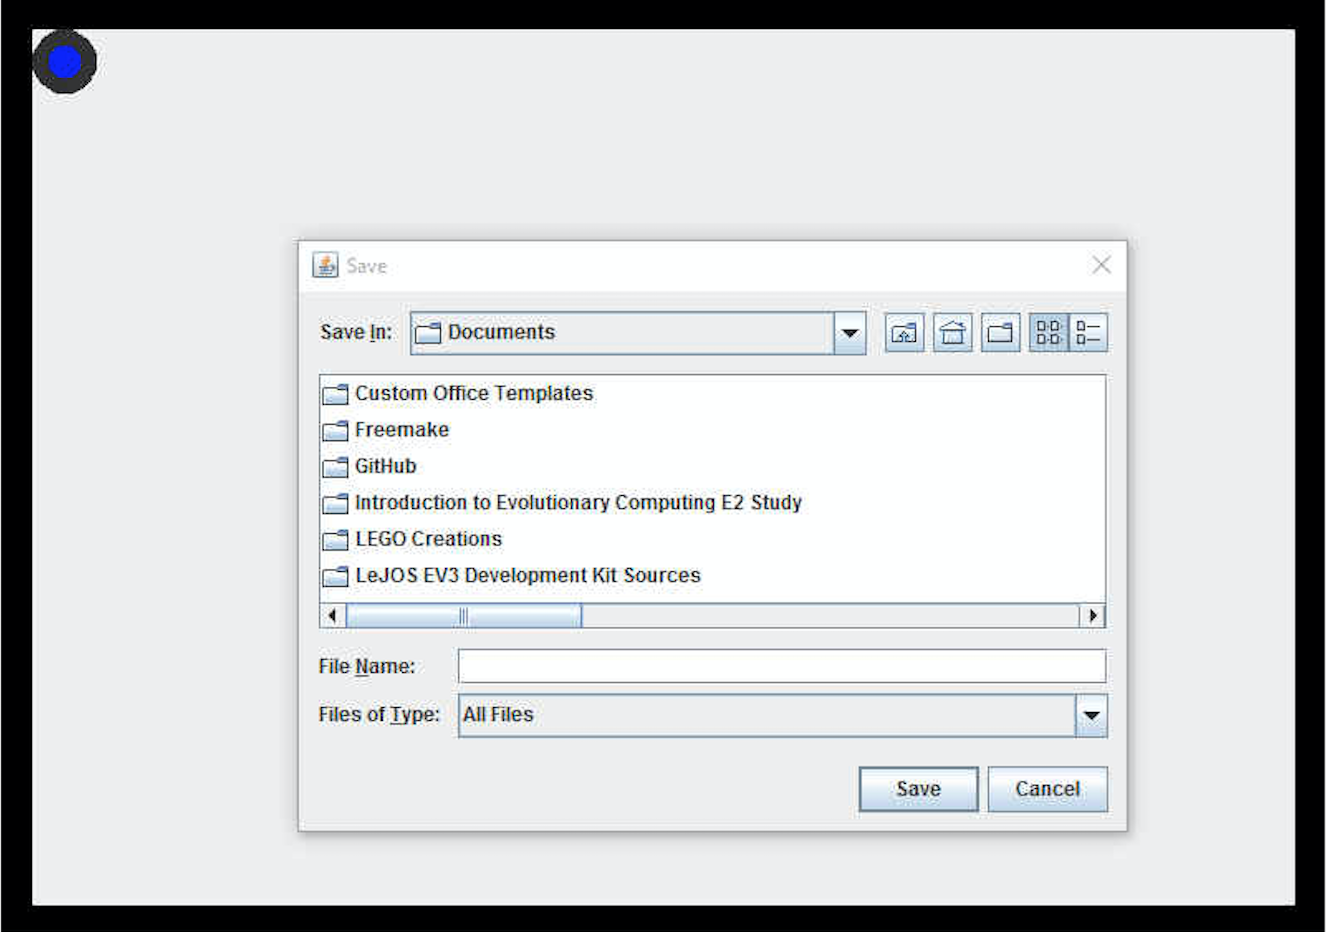
\includegraphics[height=3in]{save}
\caption[Map Save]{Map Save}
\end{figure}
\newpage

%Section 7
\section{Resource Estimates}
Our system is implemented based on the required needs from client. It should demand sufficient memory, steady storage space, an adequate CPU for the necessary application, and a bluetooth connection.\\
\\
\textbf{For PC's environment:}
\begin{itemize}
\item {The system should have or be able to have JVM 1.6 installed. }
\item {OS: }Windows, MacOSX and Linux
\item {RAM: }At least 256MB
\item {Disk Space: } At least 10MB
\item {Bluetooth communication support}
\end{itemize}
\\
\textbf{For Robot's needs:}
\begin{itemize}
\item {Robot kit: }Lego Mindstorms EV3
\item {Working plane: }A1 paper size
\item {Colour of Background: }White
\item {Colours of Deposit: } Red, yellow, blue and green
\item {Colours of Boundary and NGZ: }Black
\item {Size of Boundary and NGZ: }rectangular
\item {Size of Deposit: }circle
\end{itemize}

%Section 8
\section{Definitions, Acronyms, and Abbreviations}
\begin{itemize}
\item { SDD - }Software Design Description
\item { UML - }Unified Modelling Language
\item { SRS - }Software Design Description
\item { GUI - }Graphics Users Interface
\item { NGZ - }No-Go Zone
\item { DBMS - }Database Management System
\item { JVM - }Java Virtual Machine
\item { MB - }Megabyte
\item { RAM - }Random Access Memory
\item { CPU - }Central Processing Unit
\item { OS - }Operating System
\item { PC - }Personal Computer
\end{itemize}

\end{document}